\documentclass[UTF8, 11pt, oneside]{ctexart}

\usepackage{float}

\usepackage{geometry}
\geometry{a4paper,left=2cm,right=2cm,top=2cm,bottom=1cm}

\usepackage{graphicx}

\usepackage{hyperref}
\hypersetup{colorlinks=true, linkcolor=red}

\linespread{1.6}


\def\articletitle{印第安人的长相,很像中国人}

\usepackage{fancyhdr}
\usepackage{ifthen}
\pagestyle{fancy}
\fancyhf{}
\setlength{\headheight}{14pt}
\fancyhead[R]{\ifthenelse{\value{page}>1}{\thepage}{}}
\fancyhead[C]{\ifthenelse{\value{page}>1}{\articletitle}{}}
\renewcommand\headrulewidth{0pt}

\usepackage{tcolorbox}
\tcbuselibrary{skins}


\newcommand{\zd}[1]{\textbf{\textcolor[RGB]{123,12,0}{#1}}} % 重点

\newcommand{\yh}[1]{% 引用
    \begin{tcolorbox}[enhanced,
        frame hidden, interior hidden,
        before skip = 5mm, left skip=10mm,
        borderline west={5pt}{0pt}{gray!50}]
        #1
    \end{tcolorbox}
}

\newcommand{\biaoti}[1]{% 标题
    \section*{#1}
}

\begin{document}

\begin{center}
    \LARGE{\articletitle\footnotemark}
\end{center}
\footnotetext{
    原文出自公众号“远方青木”的文章 《\href{https://mp.weixin.qq.com/s/HcyqE5CFLtXcw6qMIUcX-g}{\articletitle}》
}

根据优胜劣汰的自然进化论,热带地区最适宜黑种人的生存,温带地区最适宜黄种人的生存,而寒带地区最适宜白种人的生存。
但是中国和美国都属于温带气候,纬度也非常相似,按理说都是最适宜黄种人生存的土地。

为何在中国生存的是黄种人,而在美国生存的是白种人。

一个11岁的小孩,提出了这个问题。

而这个小孩自行推导出了一个结论: \zd{美国的土地上,是不是换过人种了? }

\begin{figure}[H]
    \centering
    
\includegraphics[width=10cm]{2023-10-13-001}
\end{figure}

这个聪明的小孩,无意间就猜透了历史的奥秘。

\zd{美国的土地上,确实已经换了人种。}

而且是用特别血腥的手段,将原本生存在美洲大地上的黄种人,给近乎于彻底灭绝。

\biaoti{蒙古人种美洲支系}

印第安人喜欢在脸上涂抹红色颜料,这是他们的文化传统,因此欧洲白人入侵者在最开始的时候,称呼印第安人为红种人。

但实际上他们是彻彻底底的黄种人。

如今的人类学家和考古学界,已对印第安人的出身做出了明确的结论。

\zd{印第安人,是蒙古人种的美洲支系。}

为什么印第安人是蒙古人种?

因为无论是从基因溯源还是从考古证据,他们都是彻底的蒙古人种。

和中国人的血统非常的接近。

这带来的结果,就是真正的印第安人,长的和中国人非常的相似。

这是照相技术刚发明时,拍摄下来的一个真正的纯印第安女人。

你觉得像不像中国的蒙古人?

\begin{figure}[H]
    \centering
    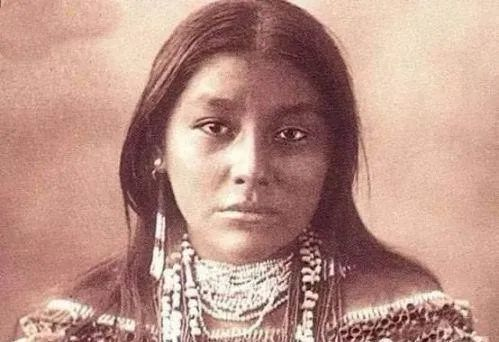
\includegraphics[width=10cm]{2023-10-13-002}
\end{figure}

还有另外一张流传下来的印第安女人照片,外貌和中国北方少数民族非常的相似。

\begin{figure}[H]
    \centering
    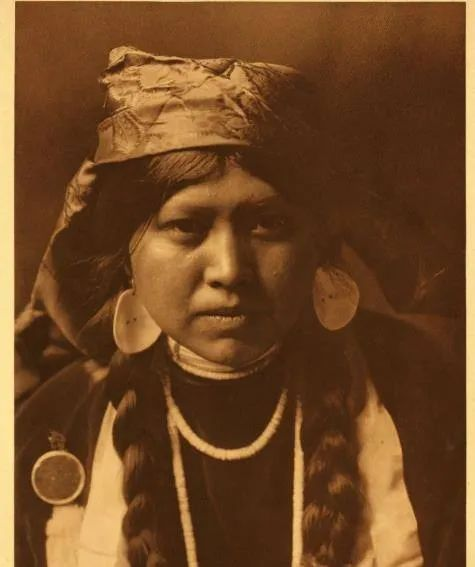
\includegraphics[width=10cm]{2023-10-13-003}
\end{figure}

古老的纯印第安人照片流传下来的不多,但今天的地球上,还残存少量的印第安人,他们有更加高清的照片。

这是印第安保留地里的舞蹈表演队,都是印第安人出演,黄种人血统特征一目了然。

\begin{figure}[H]
    \centering
    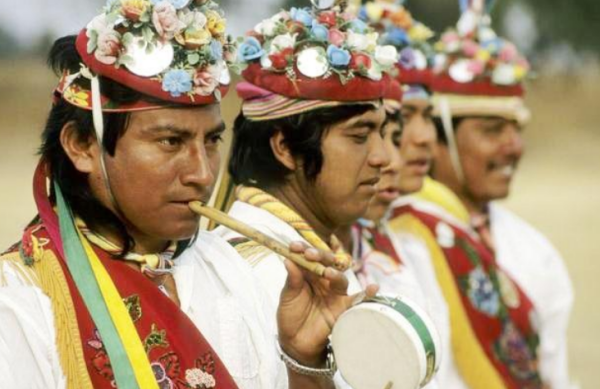
\includegraphics[width=10cm]{2023-10-13-004}
\end{figure}

而下图,是位于美国亚利桑那州的印第安保留地,Navajo部落的主政官员夫妇的照片,纯正印第安人。

你看看他们的长相,你觉得像哪国人?

\begin{figure}[H]
    \centering
    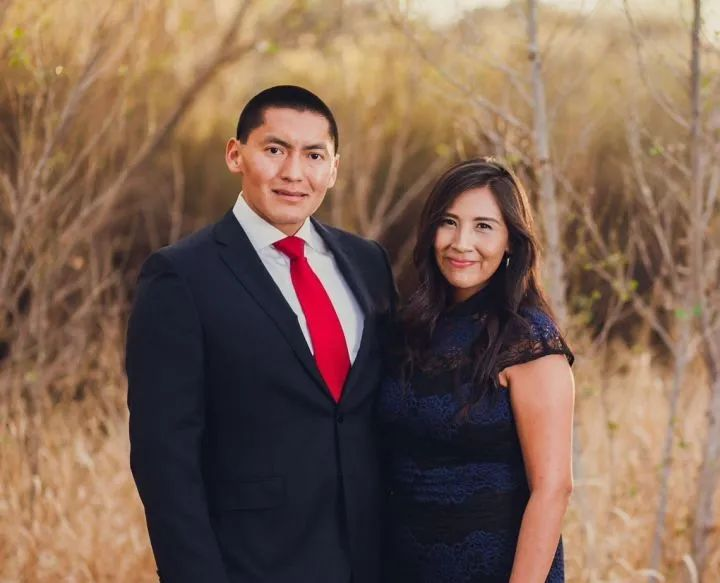
\includegraphics[width=10cm]{2023-10-13-005}
\end{figure}

换上西装后,连少数民族的风情都没了,很像我们小区里的普通邻居。

而下面这个小姑娘,是纯种的玛雅人,印第安人的一个分支,目前生活在美洲的危地马拉地区。

\begin{figure}[H]
    \centering
    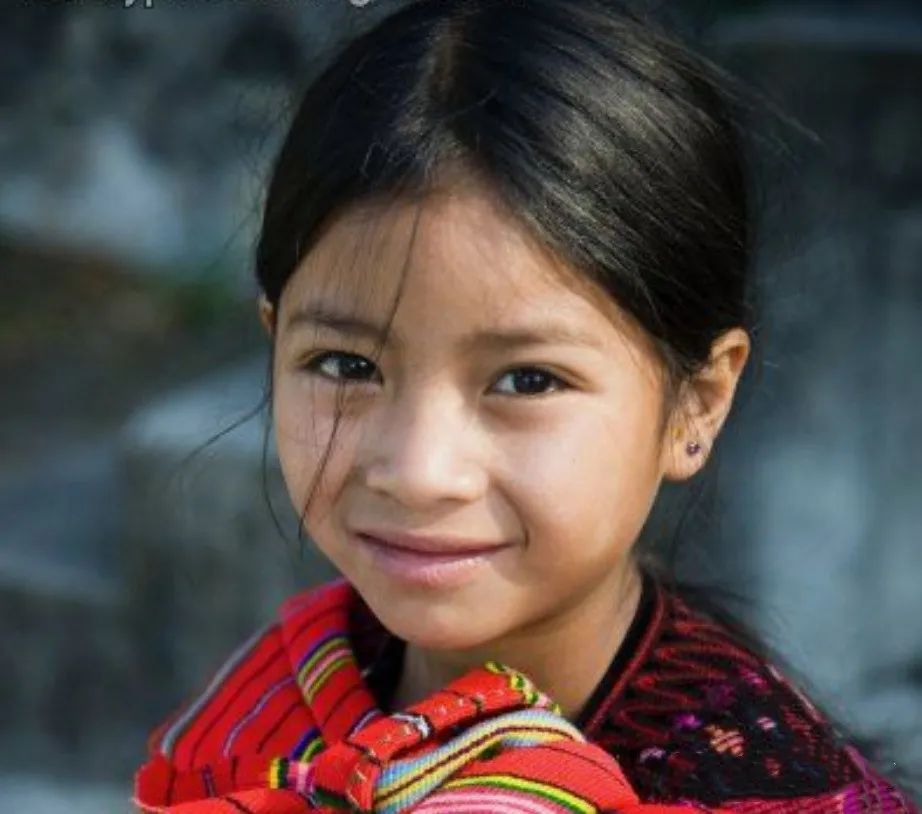
\includegraphics[width=10cm]{2023-10-13-006}
\end{figure}

\zd{纯正的黄皮肤,外加黑头发黑眼睛,如果单纯从外表上看,典型中国人。}

除此之外,对印第安人遗迹的考古,也发现了大量的中国元素。

中国有句歌词,叫“\zd{黑眼睛黑头发黄皮肤,永永远远是龙的传人}”。

巧了,古印第安人也崇拜龙图腾,在古印第安人的壁画中,考古学家发现了大量的龙状石刻。

印第安人族群里口口相传天狗吃月亮的传说,以及和大禹治水非常相似的洪水故事(人名不一样)。

而在1953美洲出土的科藩遗址墙上的印第安族鸟形王冠上,竟然发现了太极图。

除此之外,人类考古学家目前已经在美国亚利桑那州、加州、新墨西哥州、俄克拉荷马州、犹他州和内华达州的岩壁上发现了84处殷商甲骨文或中国象形文字遗迹。

对,\zd{在美国的土地上,在印第安人的古遗迹中,发现了中国殷商时期的甲骨文和象形文字。}

而且印第安人的语言,其发音习惯和音色,也和中国人有少许雷同。

目前,历史学家高度怀疑美洲印第安人中有中国的殷商后裔,但证据不够充分,仅仅84处殷商甲骨文遗迹做不到铁证如山。

但其他领域的证据是充分的。

所以,目前人类学家已形成公论,把印第安人定义为了蒙古人种美洲支系。

而中国人,也是蒙古人种的一个支系。

所以中国人和印第安人才长的如此相似。


\biaoti{对印第安人的大屠杀}

1620年,“五月花”号搭载了102名清教徒来到了美洲。

由于缺乏生存物资,这些人差点被全部冻死饿死。

这时候,善良的印第安人及时送给了他们一批粮食和生活必需品,让他们熬过了在美洲的第一个冬天。

次年开春,印第安人还教他们如何在本地狩猎、捕鱼和种植作物,帮助他们完成了定居。

到了秋季丰收时,为了感谢上帝的恩赐和印第安人的帮助,清教徒们宴请印第安人,作为救命之恩的回礼,这一天是1621年11月下旬的星期四。

后来,每年11月下旬的周四都被定为美国的法定节假日,命名为\zd{感恩节}。

欧洲殖民者和印第安人的关系本来是非常好的,但双方有一个不可调和的矛盾。

印第安人要土地,但欧洲殖民者也要土地,但只有一个人可以拿到土地。

欧洲殖民者的土地多一点,印第安人的土地就会少一点。

如果欧洲殖民者只有几十人几百人也就罢了,等几千几万殖民者定居后,巨大的矛盾会冲淡之前的一切友谊。

你能劝说欧洲殖民者放弃对土地的要求,乖乖的返回欧洲么?

当然不能。

那接下来会发生什么就很容易预测了。

1776年,美国正式建国。

为扩张国力,美国的四大国父均发表过精辟的人权论述。

华盛顿说:\zd{“用印第安人的皮可做出优质的长筒靴”。}

杰佛逊说:\zd{“美国必须灭绝印第安人”。}

罗斯福说:\zd{“只有死掉的印第安人才是好的印第安人”。}

林肯说:\zd{“美国应每10分钟屠杀一名印第安人” }

\begin{figure}[H]
    \centering
    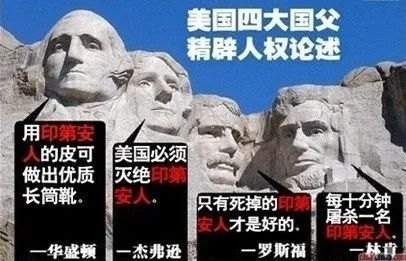
\includegraphics[width=10cm]{2023-10-13-007}
\end{figure}

除此之外,华盛顿还曾对印第安人公开发表过这样的言论:

\yh{
    “两者都是掠食的野兽,仅仅在形状上不同。”\\
    “印第安人居留地被有效摧毁前不要听取任何和平的建议。”
}

华盛顿还在打扫战场时指点过自己手下的军士:

\yh{
    “从臀部往下剥皮,这样可以制作出高的或可以并腿而长的长统靴来。”
}

1807年,美国另一位国父,第三任美国总统杰斐逊则说:

\yh{
    “如果印第安人反抗美国人去获取他们的土地,那么,对印第安人的反抗就要用短柄斧头反击,”\\
    “在战争中,他们也会杀死我们中的某些人,但我们会杀死他们全部!”
}

林肯麾下著名战将谢尔顿将军还说过一句名言:

\yh{
    今年多杀点(印第安人),明年就能少杀点。
}

1818年,美国政府正式颁布了一项法令,并通过了国会的审批。

任何美国公民,每上缴一张12岁以上印第安男子的头皮,可以获得100美元的奖励,每上缴一张印第安妇女和儿童的头皮,可以获得50美元的奖励。

200年前的印第安妇女和儿童,大概长下面这个样子。

\zd{黑头发黑眼睛,外加一身黄皮肤。}

\begin{figure}[H]
    \centering
    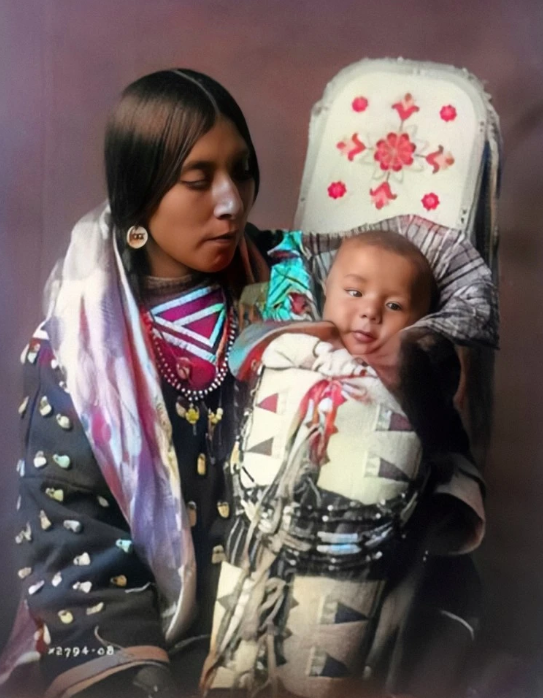
\includegraphics[width=10cm]{2023-10-13-008}
\end{figure}

\zd{只要把她们的头皮剥了,上缴给美国政府,就可以拿到2张50美元的钞票。}

自从剥皮令下达后,美国印第安人的数量急剧减少,整个美洲都是惨无人道的虐杀。

美国陆军名将谢里丹的日记里,描述了印第安人的惨状。

\yh{
    “自1862年以来,在我的辖区里至少有八百名男女和儿童惨遭杀害,其被害情况令人发指。男人通常被剥去头皮,肢体分离,他们的生殖器被凶手割下,放在他们嘴里。妇女被暴徒强奸,有时多达五六十次,然后被杀害,她们的头皮被凶手剥下,阴道里被插入棍棒,有的在她们死之前,有的在她们死之后。”
}

直到1891年,美国的纽约时报,还采访了陆军将领,将美国陆军屠杀印第安人的战绩当成“丰功伟绩”来进行大篇幅报道。

那可是1891年,光绪17年,中国马上就辛亥革命了,美国那边依然在对印第安人持续屠杀。

1900年,全美国的印第安人,只剩下了25万人。

\zd{曾经纵横整整一个美洲大陆,占领面积不亚于中国的印第安人,只剩下25万人了。}

很多人说,美国白人没杀几个人,他们都是死于天花等传染病。

但事实上,印第安人遍布整个美洲,从墨西哥一路到巴西,印第安人的比例都远远超过美国。

什么细菌病毒这么厉害,居然认美国的国境线,离开国境线的印第安人一律可以免死,新冠病毒怎么就没有这个觉悟?

美国确实有很多印第安人死于天花,但并不是自然感染。

1763年,美洲英军总指挥官杰弗里·阿默斯特曾公开表示:

\yh{
    将带有天花病菌的毛毯送给原住民部落是值得赞美的创举。
}

美洲有大量印第安人也持有枪支,杀起来有点困难,但利用医学知识的优势,大量赠送带毒物品,用人造瘟疫的办法悄悄灭杀对方整个族群,就简单了很多。

生化战的典范。

\begin{figure}[H]
    \centering
    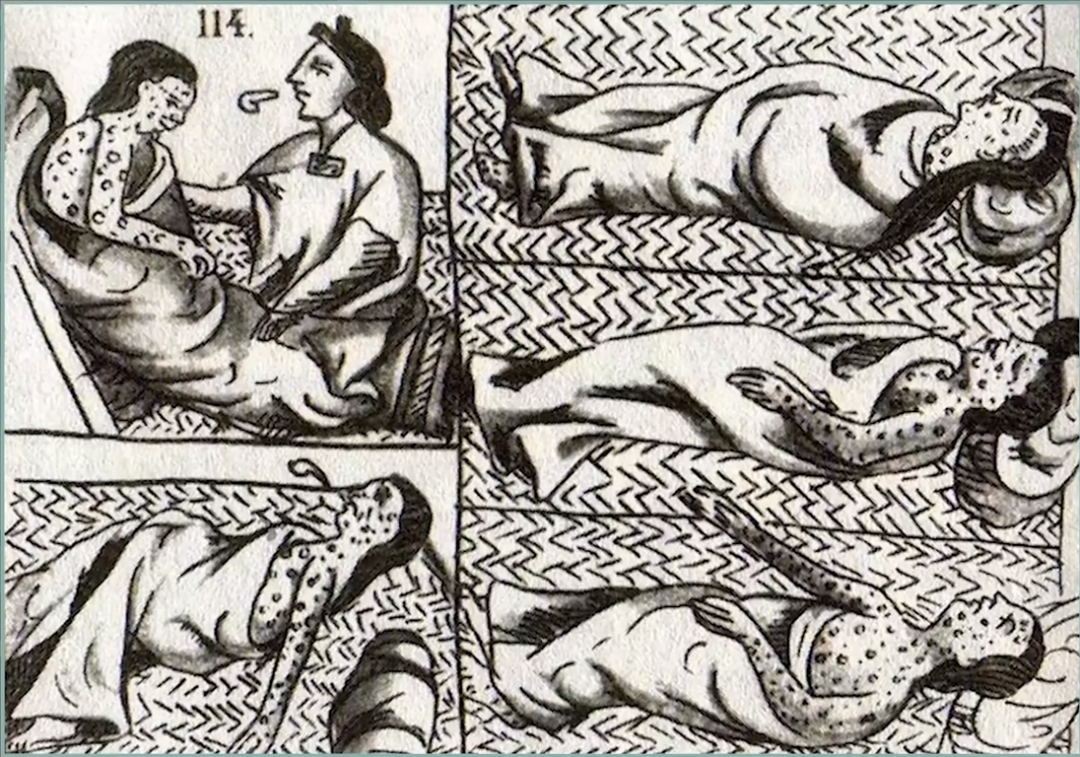
\includegraphics[width=10cm]{2023-10-13-009}
\end{figure}

等到了后期印第安人知道如何对付传染病的办法后,华盛顿等人,就只能用野蛮的办法,硬生生的一点点去屠杀。

最终,几乎杀绝了印第安人。

只剩25万,只剩25万啊!

\zd{长相和中国人差不多,地盘和中国也差不多大的印第安人族群,}被屠杀了3个世纪后,只剩下了25万人。


\biaoti{投降无意义 }

印第安人被杀的那么惨,是不是因为印第安人疯狂抵抗的原因,如果全民投降欧洲殖民者行不行。

事实上,印地安人中一直存在大量的投降派,并有大量的人亲近欧洲殖民者。

而印第安人中的主战派,其战斗力也给欧洲殖民者带来了巨大的麻烦,让欧洲殖民者觉得有拉拢分化印第安人的必要性。

正是这两者的同时存在,灭绝印第安人才用了足足3个世纪。

因为欧洲殖民者内部的声音也很分裂,一部分人觉得应该消灭部分强硬印第安人,保留友善的印第安人,而另一部分人觉得应该无差别全部消灭。

而且欧洲殖民者自己的人口也太少,土地扩张的太快,人口增殖需要时间,短期消化不了太多土地。

既然短期内太多土地无意义,印第安人的抵抗有很有威慑力,同时还有主和派制约,那就把战争停一停。

这导致对印第安人的政策,是打打停停。

但最终,种族主义还是在漫长的历史长河中占据了上风,消灭掉了印第安和平派的努力,并最终灭绝了几乎所有的印第安人。

因为人口大量繁衍后的美国白人,需要更多生存的土地,这就必然和原本已经达成和平协定的印第安人产生巨大的冲突。

\zd{所以最终,不管你是主战派还是投降派,结果都是个死。}

也许投降派生前的几十年里,其麾下的印第安人只是生存恶劣了点,最终还是可以活下去的。

\zd{但3个世纪后,所有投降派的后代,只活下来了25万人。}

包含所有男女老幼,曾经占据一个大陆的庞大族群的所有后代。

怎么死的不重要,美国政府给出的官方理由你听听就行了,反正各种各样的理由都有,但最终结果就是几乎全死了,而美国白人种族则膨胀到了以亿为单位的人口数量。

希特勒被骂的那么惨,其实也就只杀了1/3的犹太人而已,论比例,美国人灭绝印第安人的力度要恐怖的多。

美国发展史,就是一部印第安人血泪史。

现代社会承平日久,很多人对战争产生了错觉。

比如说有人认为军队一定会维持良好的军纪,绝不会滥杀无辜。

比如说有人觉得平民不会成为战争目标。

比如说有人觉得战俘一定会得到善待。

比如说有人认为女人和战争没有关系。

真的是很幼稚。

自从人类发明核弹后,核威慑让地球上已经很久很久没有爆发过残酷的国家总体战了,让很多人产生了不切实际的幻觉。

就以女人和战争没有关系这一点来说。

抗日的时候,鬼子一来所有的女性都要在脸上抹锅底灰并到处躲藏,你以为她们在躲什么?

\zd{战争中让女人走开},这是本方男性的责任和义务,\zd{是一种目标,但并不是必然。}

想实现这个目标,一定是建立在本方男性打赢的基础上。

如果本方男性打输了,女人是不可能走开的,也跑不掉。

印第安人的黄种女人,头皮价值50美元一个,无论来源。

\zd{不管你是否美丑,不管你对白人是否亲善,总会有缺钱的白人对你下手的。}

至于投降的印第安女人,数量很多,但活下来的不多,因为印第安人的后代存活总数摆在那里。

再说个近一点的,印尼反华的时候,华人男性全部杀光,而华人女性你以为只是被侮辱就完了么?

并不是,轮奸完直接用螺纹钢筋从下体穿进去,慢慢弄死。

\zd{这不是意淫文学,而是史实,}类似的图片甚至是视频都很多,只不过由于过于血腥都被和谐了,有兴趣的可以自己搜索下。

\zd{种族不同,文化不同的情况下,一旦战败,下场实在是太惨了。}

不要幻想依靠别人来伸张正义,也不要幻想自己的抗议有效。

\zd{只要把原住民杀绝了,自然就没人抗议了。}

现在国际人权届的三大旗手,美国加拿大和澳大利亚,其统治族群都是白人,但白人都不是这些国家的原住民。

美国的原住民是印第安人,加拿大那么大的领土自然是有原住民的,澳大利亚那么大的领土自然也是有原住民的。

那你说说加拿大和澳大利亚上面的原住民在哪,人呢?

因为美国当初还保留了几十万印第安人,后来繁衍到了几百万,所以到今天还有印第安人不断的为自己伸冤。

因为希特勒还有2/3的犹太人没杀,所以到今天都有犹太人持续抨击希特勒。

加拿大和澳大利亚倒是耳根子清静,指责他们屠杀原住民的声音非常的小。

\zd{外人毕竟事不关己,偶尔提一下已经很不错了,反正被屠杀的又不是自己的族人。}

欧洲殖民者来到美洲的时候,印第安人对他们说:

\yh{
    “既然你们在此地是陌生人,来到我们的领土后,应该让自己入乡随俗,遵守我们的习惯,而不是将你们的习俗强加于我们。”
}

欧洲殖民者确实没有打算把自己的习俗强加给印第安人,因为他们选择了直接灭绝印第安人的肉体,这样更省事。

杀人不要紧的,\zd{以后照样可以成为代表人权和文明的灯塔。}

\zd{因为历史是由胜利者书写的,而胜利者永远是正确的。 }

\end{document}

